\حصہ{غیر منفی اجزاء والے تسلسل کا تکملی پرکھ}
ہم تسلسل \عددی{\sum a_n} کے بارے میں دو سوالات کرتے ہیں:
\begin{enumerate}[a.]
\item
کیا یہ تسلسل مرتکز ہے؟
\item
اگر تسلسل مرتکز ہو تب اس کا مجموعہ کیا ہے؟
\end{enumerate}

اس باب کا باقی بیشتر حصہ پہلے سوال کا جواب دے گا۔ حقیقتاً دوسرا سوال بھی اتنا ہی اہم ہے اور ہم اس پر بعد میں غور کریں گے۔

اس حصہ میں اور اگلے دو حصوں میں ایسے تسلسل پر غور کیا جائے گا جن میں منفی اجزاء نہیں پائے جاتے ہوں۔ اس شرط کی بنا ان تسلسل کے جزوی مجموعے غیر گھٹتے ترتیبات دیتے ہیں اور وہ غیر گھٹتے ترتیبات جو  اوپر سے محدود ہوں ہر صورت مرتکز ہوتے ہیں (مسئلہ \حوالہ{مسئلہ_تسلسل_غیر_گھٹتا_تسلسل})۔ یہ دکھانے کی خاطر کہ ایک غیر منفی اجزاء والا تسلسل مرتکز ہے، ہمیں صرف اتنا دکھانا ہو گا کہ اس تسلسل کے جزوی مجموعے اوپر سے محدود ہیں۔

ابتدا میں یوں معلوم ہوتا ہے جیسے اس ترکیب سے ارتکاز کی تصدیق کرنے کے باوجود تسلسل کا مجموعہ نہ جاننا ایک عیب ہے۔ کیا بہتر ہوتا کہ ہم جزوی مجموعوں کے کلیات سے تسلسل کا مجموعہ بلا واسطہ تلاش کرتے۔ حقیقت میں ہمیں عموماً جزوی مجموعوں کے کلیات معلوم نہیں ہوں گے  اور اسی بنا ہمیں دو قدمی طریقہ کار استعمال کرنا ہو گا جہاں پہلے قدم میں تسلسل کا ارتکاز جانا جاتا ہے اور دوسرے قدم میں مجموعے کی تخمینی قیمت تلاش کی جاتی ہے۔ 

\جزوحصہء{غیر گھٹتے جزوی مجموعے}
فرض کریں کہ تمام \عددی{n} کے لئے \عددی{a_n\ge 0} ہو اور \عددی{\sum_{n=1}^{\infty}a_n} لامتناہی تسلسل ہو۔
 تب چونکہ \عددی{s_{n+1}=s_n+a_n} ہے لہٰذا ہر جزوی مجموعہ گزشتہ جزوی مجموعے سے بڑا یا اس کے برابر ہو گا:
\begin{align*}
s_1\le s_2\le s_3\le \cdots\le s_n\le s_{n+1}\le \cdots
\end{align*}
اب جزوی مجموعے غیر گھٹتا ترتیب بناتے ہیں اور مسئلہ \حوالہ{مسئلہ_تسلسل_غیر_گھٹتا_تسلسل} کے تحت یہ تسلسل صرف اور صرف اس صورت مرتکز ہو گا جب اس کے جزوی مجموعات اوپر سے محدود ہوں۔

\ابتدا{ضمنی نتیجہ} برائے مسئلہ \حوالہ{مسئلہ_تسلسل_غیر_گھٹتا_تسلسل}
غیر منفی اجزاء کا تسلسل \عددی{\sum_{n=1}^{\infty}a_n} صرف اور صرف اس صورت مرتکز ہو گا جب اس کے جزوی مجموعات اوپر سے محدود ہوں۔
\انتہا{ضمنی نتیجہ}
%=========================

\ابتدا{مثال}\ترچھا{ہارمونی تسلسل}\\
درج ذیل تسلسل کو \اصطلاح{ہارمونی تسلسل}\فرہنگ{تسلسل!ہارمونی}\حاشیہب{harmonic series}\فرہنگ{series!harmonic} کہتے ہیں۔
\begin{align*}
\sum_{n=1}^{\infty}\frac{1}{n}=1+\frac{1}{2}+\frac{1}{3}+\cdots+\frac{1}{n}+\cdots
\end{align*}
اس کے جزوی مجموعوں کی کوئی بالائی حد بندی نہیں پائی جاتی ہے لہٰذا یہ  مرتکز  تسلسل ہے۔ اس حقیقت کو جاننے کی خاطر ہم اجزاء کے گروہ بناتے ہیں۔
\begin{align*}
1+\frac{1}{2}+\underbrace{\big(\frac{1}{3}+\frac{1}{4}\big)}_{>\tfrac{2}{4}=\tfrac{1}{2}}+\underbrace{\big(\frac{1}{5}+\frac{1}{6}+\frac{1}{7}+\frac{1}{8}\big)}_{>\tfrac{4}{8}=\tfrac{1}{2}}+\underbrace{\big(\frac{1}{9}+\frac{1}{10}+\cdots+\frac{1}{16}\big)}_{>\tfrac{8}{16}=\tfrac{1}{2}}+\cdots
\end{align*}
پہلے دو اجزاء کا مجموعہ \عددی{1.5} ہے۔اگلے دو اجزاء کا مجموعہ \عددی{\tfrac{1}{3}+\tfrac{1}{4}} ہے جو \عددی{\tfrac{1}{4}+\tfrac{1}{4}=\tfrac{1}{2}} سے بڑا ہے۔ اگلے چار اجزاء کا مجموعہ \عددی{\tfrac{1}{5}+\tfrac{1}{6}+\tfrac{1}{7}+\tfrac{1}{8}} ہے جو \عددی{\tfrac{1}{8}+\tfrac{1}{8}+\tfrac{1}{8}+\tfrac{1}{8}=\tfrac{1}{2}} سے بڑا ہے۔ اگلے آٹھ اجزاء کا مجموعہ
 \عددی{\tfrac{1}{9}+\tfrac{1}{10}+\tfrac{1}{11}+\tfrac{1}{12}+\tfrac{1}{13}+\tfrac{1}{14}+\tfrac{1}{15}+\tfrac{1}{16}} ہے جو  \عددی{\tfrac{1}{16}+\tfrac{1}{16}+\tfrac{1}{16}+\tfrac{1}{16}+\tfrac{1}{16}+\tfrac{1}{16}+\tfrac{1}{16}+\tfrac{1}{16}=\tfrac{1}{2}} سے بڑا ہے۔ اسی طرح اگلے سولہ اجزاء کا مجموعہ بھی \عددی{\tfrac{1}{2}} سے بڑا ہو گا، وغیرہ وغیرہ۔ یوں جزو \عددی{\tfrac{1}{2^{n+1}}} پر اختتام پذیر  \عددی{2^n} اجزاء کا مجموعہ \عددی{\tfrac{2^n}{2^{n+1}}=\tfrac{1}{2}} سے بڑا ہو گا۔جزوی مجموعات کی ترتیب اوپر سے محدود نہیں ہے: اگر \عددی{n=2^k} ہو تب جزوی مجموعہ \عددی{s_n} کی قیمت \عددی{\tfrac{k}{2}} سے بڑی ہو گی۔ ہارمونی تسلسل منفرج ہے۔
\انتہا{مثال}
%===========================

دھیان رہے کہ ہارمونی تسلسل کا \عددی{n} واں جزو \عددی{\tfrac{1}{n}} ہے جو \عددی{0} پر مرتکز ہے لیکن ہارمونی تسلسل منفرج ہے۔یوں ہارمونی تسلسل کے انفراج کو دریافت کرنے میں انفراج کا \عددی{n} ویں جزو پرکھ  نا کام  ہوتا ہے۔

\جزوحصہء{تکملی پرکھ}
ہم ہارمونی تسلسل سے تعلق رکھنے والے ایک تسلسل، جس کا \عددی{n} واں جزو \عددی{\tfrac{1}{n^2}} ہے، کو استعمال کرتے ہوئے تکملی پرکھ کو متعارف کرتے ہیں۔

\ابتدا{مثال}\شناخت{مثال_تسلسل_مرتکز_تسلسل_موازنہ_تکمل}
کیا درج ذیل تسلسل مرتکز ہے؟
\begin{align*}
\sum_{n=1}^{\infty}\frac{1}{n^2}=1+\frac{1}{4}+\frac{1}{9}+\frac{1}{16}+\cdots+\frac{1}{n^2}+\cdots
\end{align*}
حل:\quad
ہم \عددی{\int_1^{\infty}\tfrac{\dif x}{x^2}} کے ساتھ موازنہ کرتے ہوئے \عددی{\sum_{n=1}^{\infty}\tfrac{1}{n^2}} کی ارتکاز دریافت کرتے ہیں۔ موازنہ کرنے کی خاطر ہم تسلسل کے اجزاء کو تفاعل \عددی{f(x)=\tfrac{1}{x^2}} کی قیمتیں تصور کرتے ہیں اور ان قیمتوں کو منحنی \عددی{y=\tfrac{1}{x^2}} کے نیچے مستطیل رقبے تصور کرتے ہیں۔

جیسا شکل \حوالہ{شکل_مثال_تسلسل_مرتکز_تسلسل_موازنہ_تکمل} میں دکھایا گیا ہے درج ذیل ہو گا۔
\begin{align*}
s_n&=\frac{1}{1^2}+\frac{1}{2^2}+\frac{1}{3^2}+\cdots+\frac{1}{n^2}\\
&=f(1)+f(2)+f(3)+\cdots+f(n)\\
&<f(1)+\int_1^{n}\frac{1}{x^2}\dif x\\
&<1+\int_1^{\infty}\frac{1}{x^2}\dif x\\
&<1+1=2&&\text{\RL{(مثال \حوالہ{مثال_طریقہ_منحنی_کے_نیچے_رقبہ_متناہی_یا_نہیں})}}
\end{align*}
یوں \عددی{\sum_{n=1}^{\infty}\tfrac{1}{n^2}} کے جزوی مجموعات اوپر سے (\عددی{2} تک) محدود ہیں لہٰذا یہ تسلسل مرتکز ہو گا۔  اس تسلسل کا مجموعہ درحقیقت \عددی{\tfrac{\pi^2}{6}\approx 1.64493} ہے۔
\انتہا{مثال}
%=======================
\begin{figure}
\centering
\begin{tikzpicture}[font=\small,declare function={f(\x)=1/(\x^2);}]
\begin{axis}[clip=false,small,axis lines=middle,xlabel={$x$},ylabel={$y$},xlabel style={at={(current axis.right of origin)},anchor=west},ylabel style={at={(current axis.above origin)},anchor=south},xmin=0,ymin=0,ytick={\empty},xtick={1,2,3,4,7,8},xticklabels={$1$,$2$,$3$,$4$,$n-1$,$n$}]
\addplot[smooth,domain=0.9:9]{f(x)};
\draw(0,{f(1)})--(1,{f(1)})node[right]{$(1,f(1))$}--(1,0);
\draw(1,{f(2)})--(2,{f(2)})node[pin={[pin distance=1cm]70:{$(2,f(2))$}}]{}--(2,0);
\draw(2,{f(3)})--(3,{f(3)})node[pin={[pin distance=1cm]50:{$(3,f(3))$}}]{}--(3,0);
\draw(3,{f(4)})--(4,{f(4)})--(4,0);
\draw(1/2,{1/2*f(1)})node[]{$\tfrac{1}{1^2}$};
\draw(1+1/2,{1/2*f(2)})node[]{$\tfrac{1}{2^2}$};
\draw(2.2,{1/3*f(3)})node[pin=60:{$\tfrac{1}{3^2}$}]{};
\draw(3.2,{1/4*f(4)})node[pin=30:{$\tfrac{1}{4^2}$}]{};
\draw(8,{f(8)})node[pin=45:{$(n,f(n))$}]{};
\draw(7.5,{0})node[pin=70:{$\tfrac{1}{n^2}$}]{};
\draw(7,{f(1)})node[]{$f(x)=\frac{1}{x^2}$};
\end{axis}
\end{tikzpicture}
\caption{رقبہ کا موازنہ (مثال \حوالہ{مثال_تسلسل_مرتکز_تسلسل_موازنہ_تکمل})}
\label{شکل_مثال_تسلسل_مرتکز_تسلسل_موازنہ_تکمل}
\end{figure}

\موٹا{تکملی پرکھ}\\
فرض کریں \عددی{\{a_n\}} مثبت اجزاء کی ترتیب ہے۔ مزید فرض کریں کہ \عددی{a_n=f(n)} ہے جہاں تمام \عددی{x\ge N} کے لئے ( \عددی{N} مثبت عدد صحیح ہے)  متغیر \عددی{x} کا \عددی{f}  استمراری، مثبت اور گھٹتا تفاعل ہے۔ تب تسلسل \عددی{\sum_{n=N}^{\infty}a_n} اور تکمل \عددی{\int_N^{\infty}f(x)\dif  x} دونوں مرتکز یا دونوں منفرج ہوں گے۔

\ابتدا{ثبوت}
ہم \عددی{N=1} کے لئے پہلے اس پرکھ کو ثابت کرتے ہیں۔ عمومی \عددی{N} کے لئے ثبوت اسی طرح کا ہے۔ 

ہم اس مفروضہ سے شروع کرتے ہیں کہ تمام \عددی{n} کے لئے \عددی{f} گھٹتا تفاعل  اور \عددی{f(n)=a_n} ہیں۔ یوں شکل-الف میں وہ مستطیل جن کے رقبے \عددی{a_1,a_2,\cdots,a_n}  ہیں کا مجموعی رقبہ، \عددی{x=1} تا \عددی{x=n+1} ترسیم \عددی{y=f(x)} کے نیچے رقبہ سے زیادہ ہے یعنی:
\begin{align*}
\int_1^{n+1}f(x)\dif x\le a_1+a_2+\cdots+a_n
\end{align*} 
شکل-ب میں مستطیلوں کو ہر نقطہ کے بائیں جانب بنایا گیا ہے۔ اگر ہم وقتی طور پر پہلی مستطیل، جس کا رقبہ \عددی{a_1} ہے، کو نظر انداز کریں تب درج ذیل ہو گا۔
\begin{align*}
a_2+a_3+\cdots+a_n\le \int_1^nf(x)\dif x
\end{align*}
اگر ہم \عددی{a_1} کو بھی شامل کریں تب درج ذیل لکھا جا سکتا ہے۔
\begin{align*}
a_1+a_2+a_3+\cdots+a_n\le a_1+\int_1^nf(x)\dif x
\end{align*}
ان نتائج سے 
\begin{align}
\int_1^{n+1}f(x)\dif x\le a_1+a_2+\cdots+a_n\le  a_1+\int_1^nf(x)\dif x
\end{align}
حاصل ہوتا ہے۔ اگر \عددی{\int_1^{\infty}f(x)\dif x} متناہی ہو تب دائیں عدم مساوات کے تحت \عددی{\sum a_n} متناہی ہو گا۔  اگر \عددی{\int_1^{\infty}f(x)\dif x} لامتناہی ہو تب بائیں عدم مساوات کے تحت \عددی{\sum a_n} لامتناہی ہو گا۔ 

یوں تسلسل اور تکمل دونوں مرتکز یا دونوں منفرج ہوں گے۔
\انتہا{ثبوت}
%=======================

دھیان رہے کہ ارتکاز کی صورت میں تکمل اور تسلسل کی قیمتیں مختلف ہو سکتی ہیں جیسا مثال \حوالہ{مثال_تسلسل_مرتکز_تسلسل_موازنہ_تکمل} میں دیکھا گیا جہاں \عددی{\sum_{n=1}^{\infty}\tfrac{1}{n^2}=\tfrac{\pi^2}{6}} اور \عددی{\int_1^{\infty}\tfrac{1}{x^2}\dif x=1} تھے۔

\ابتدا{مثال}
دکھائیں کہ \عددی{p} تسلسل
\begin{align}
\sum_{n=1}^{\infty}\frac{1}{n^p}=\frac{1}{1^p}+\frac{1}{2^p}+\frac{1}{3^p}+\cdots+\frac{1}{n^p}+\cdots
\end{align}
جہاں \عددی{p} حقیقی مستقل ہے، \عددی{p>1} کی صورت میں مرتکز جبکہ \عددی{p\le 1} کی صورت میں منفرج ہو گا۔

حل:\quad
اگر \عددی{p>1} ہو تب \عددی{f(x)=\tfrac{1}{x^p}} متغیر \عددی{x} کا مثبت گھٹتا تفاعل ہو گا۔ اب چونکہ
\begin{align*}
\int_1^{\infty}\frac{1}{x^p}\dif x&=\int_1^{\infty}x^{-p}\dif x=\lim_{b\to\infty}\big[\frac{x^{-p+1}}{-p+1}\big]_1^b\\
&=\frac{1}{1-p}\lim_{b\to\infty}(\frac{1}{b^{p-1}}-1)\\
&=\frac{1}{1-p}(0-1)=\frac{1}{p-1}
\end{align*}
ہے لہٰذا تکملی پرکھ کے تحت یہ تسلسل مرتکز ہو گا۔

اگر \عددی{p<1}ہو تب \عددی{1-p>0} ہو گا لہٰذا درج ذیل لکھا جا سکتا ہے۔
\begin{align*}
\int_1^{\infty}\frac{1}{x^p}\dif x=\frac{1}{1-p}\lim_{b\to\infty}(b^{1-p}-1)=\infty
\end{align*}
تکملی پرکھ کے تحت یہ تسلسل منفرج ہو گا۔

اگر \عددی{p=1} ہو تب درج ذیل منفرج (ہارمونی) تسلسل پایا جائے گا۔
\begin{align*}
1+\frac{1}{2}+\frac{1}{3}+\cdots+\frac{1}{n}+\cdots
\end{align*} 
یوں \عددی{p>1} لے ارتکاز  لیکن \عددی{p<1} اور \عددی{p=0} کے لئے انفراج پایا جاتا ہے۔
\انتہا{مثال}
%=====================

\حصہء{سوالات}

